%%% Preamble starts here.
\documentclass{amsart}
%for the heading
\usepackage{fancyhdr, enumerate}
%for the picture. 
\usepackage{tikz, calc}
%adjust the page width
\usepackage[margin=1in]{geometry}

%% The next line says how the "vertex" style of nodes should look: drawn as small circles.
\tikzstyle{vertex}=[circle, draw, inner sep=0pt, minimum size=6pt]
%%
%% Next, we make a \vertex command as a shorthand in place of \node[vertex} to get that style.
\newcommand{\vertex}{\node[vertex]}

\usetikzlibrary{graphs}
\usetikzlibrary{graphs.standard}



\linespread{1.1}

%command for double parentheses
\newcommand{\textmultiset}[2]{\bigl(\!{\binom{#1}{#2}}\!\bigr)}
\newcommand{\displaymultiset}[2]{\left(\!{\binom{#1}{#2}}\!\right)}
\newcommand\multiset[2]{\mathchoice{\displaymultiset{#1}{#2}}
                                {\textmultiset{#1}{#2}}
                                {\textmultiset{#1}{#2}}
                                {\textmultiset{#1}{#2}}}

%special commands for number sets
\def\RR{{\mathbb R}}
\def\NN{{\mathbb N}}
\def\ZZ{{\mathbb Z}}
\def\QQ{{\mathbb Q}}
\def\CC{{\mathbb C}}

% header
\lhead{\sc  Combinatorics: Homework 10}
\chead{\sc Stefano Fochesatto } 
\rhead{\today}
\cfoot{}
\pagestyle{fancy}

%%%% Main document starts here.

\begin{document}
\thispagestyle{fancy}
 1,2,7,a,b
\begin{enumerate}
%%%first problem
\item (Problem 6.1.2) Let $G$ be the graph whose vertex set is the set of 2-subsets of $[5]$ and where two vertices are adjacent if and only if their corresponding subsets are disjoint.\\

(a) Draw $G$.\\
 
 Two vertices are drawn. You finish the picture.\\
\begin{align*}
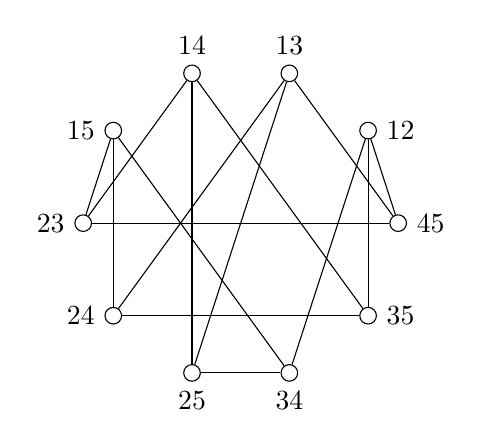
\begin{tikzpicture}
\vertex (12) at (36:2) [label=right:$12$] {};
\vertex (13) at (72:2) [label=above:$13$] {};
\vertex (14) at (108:2) [label=above:$14$] {};
\vertex (15) at (144:2) [label=left:$15$] {};
\vertex (23) at (180:2) [label=left:$23$] {};
\vertex (24) at (216:2) [label=left:$24$] {};
\vertex (25) at (252:2) [label=below:$25$] {};
\vertex (34) at (288:2) [label=below:$34$] {};
\vertex (35) at (324:2) [label=right:$35$] {};
\vertex (45) at (360:2) [label=right:$45$] {};
\draw (12)--(34);
\draw (12)--(35);
\draw (12)--(45);
\draw (13)--(24);
\draw (13)--(25);
\draw (13)--(45);
\draw (14)--(23);
\draw (14)--(25);
\draw (14)--(35);
\draw (15)--(23);
\draw (15)--(24);
\draw (15)--(34);
\draw (23)--(45);
\draw (24)--(35);
\draw (25)--(34);
%\draw (12)--(45)--(13)--(25)--(14)--(35)--(24)--(13)--(45)--(23)--(14)--(25)--(34)--(15)--(24)--(15)--(23);
\end{tikzpicture}
\end{align*}
\vspace{.2 in}

(b) Find, with proof, a graph mentioned in this section that isomorphic to $G.$\\

Consider the Peterson graph shown in p.229.

\begin{align*}
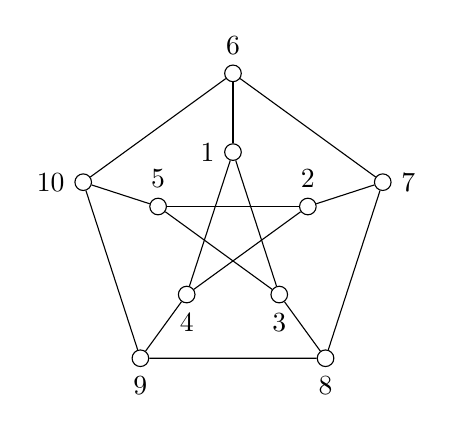
\begin{tikzpicture}
\vertex (1) at (90:1) [label=left:$1$] {};
\vertex (2) at (18:1) [label=above:$2$] {};
\vertex (3) at (306:1) [label=below:$3$] {};
\vertex (4) at (234:1) [label=below:$4$] {};
\vertex (5) at (162:1) [label=above:$5$] {};
\vertex (6) at (90:2) [label=above:$6$] {};
\vertex (7) at (18:2) [label=right:$7$] {};
\vertex (8) at (306:2) [label=below:$8$] {};
\vertex (9) at (234:2) [label=below:$9$] {};
\vertex (10) at (162:2) [label=left:$10$] {};
\draw (1)--(4);
\draw (1)--(3);
\draw (1)--(6);
\draw (2)--(5);
\draw (2)--(4);
\draw (2)--(7);
\draw (3)--(5);
\draw (3)--(8);
\draw (4)--(9);
\draw (5)--(10);
\draw (6)--(7)--(8)--(9)--(10)--(6);
\end{tikzpicture}
\end{align*}
To prove isomorphism it is not enough for both graphs to have the same number of edges, vertices, and degree sequences but it is a good start. We can see that both $G$ and the Peterson graphs are $K_{10,3}$ which tells us that there is a possibility that they are isomorphic. To show that these two graphs are isomorphic we need to prove that for $G[V_1,E_1]$ and $P[V_2,E_2]$(Peterson Graph) there is a bijection, $f : V_1\to V_2$ such that for every $\{v_1,v_2\} \in E_1$ then $\{f(v_1),f(v_2)\} \in E_2$. Consider the following graph that provides a bijection between vertices of $P$ and $G$,

\begin{align*}
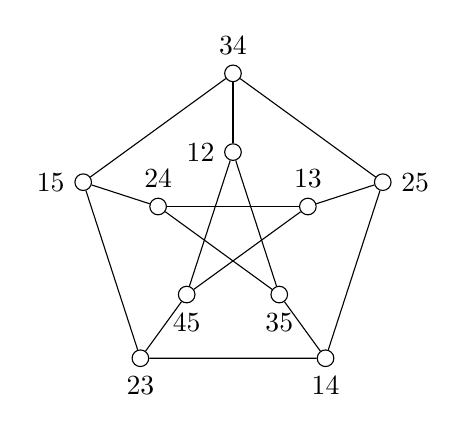
\begin{tikzpicture}
\vertex (12) at (90:1) [label=left:$12$] {};
\vertex (13) at (18:1) [label=above:$13$] {};
\vertex (35) at (306:1) [label=below:$35$] {};
\vertex (45) at (234:1) [label=below:$45$] {};
\vertex (24) at (162:1) [label=above:$24$] {};
\vertex (34) at (90:2) [label=above:$34$] {};
\vertex (25) at (18:2) [label=right:$25$] {};
\vertex (14) at (306:2) [label=below:$14$] {};
\vertex (23) at (234:2) [label=below:$23$] {};
\vertex (15) at (162:2) [label=left:$15$] {};
\draw (12)--(45);
\draw (12)--(35);
\draw (12)--(34);
\draw (13)--(24);
\draw (13)--(45);
\draw (13)--(25);
\draw (35)--(24);
\draw (35)--(14);
\draw (45)--(23);
\draw (24)--(15);
\draw (34)--(25)--(14)--(23)--(15)--(34);
\end{tikzpicture}
\end{align*}
Thus the two graphs $P$ and $G$ are isomorphic.
\vspace{.5in}

\item (Problem 6.2.1) Prove: A forest with $n$ vertices and $k$ components has $n-k$ edges. Explain how this generalizes Theorem 6.2.3.\\

\textbf{Proof:} Theorem 6.2.3 states that any tree on $n$ vertices contains exactly $n-1$ edges. Now consider a tree on $n$ vertices, by Theorem 6.2.3 it must have $n-1$ edges. If we wanted to make our tree into a forest all we would have to do is remove one edge, and this is because trees are defined as acyclic and connected so when we remove exactly one edge we create two separate trees, or two components to a forest. So in order to transform our tree on $n$ vertices with $n-1$ edges into a forest with $n$ vertices and $k$ components we must remove $k-1$ edges. Through some algebra we can see that the total number of edges comes out to, $n-1-(k-1) = n-k$. 

\vspace{1in}

\item (Problem 6.2.2) Improve Theorem 6.2.1 by proving that any tree has at least $\Delta$ leaves, where $\Delta$ is the maximum degree in the graph.\\

\textbf{Proof:} Theorem 6.2.1 states that if $T$ is a tree with at least two vertices then $T$ has at least two leaves. Now suppose we have a tree $T$ with a vertex $v$ that has degree $\Delta$. Now let's consider the forest $F$ that is created when we remove that vertex $v$ and all the edges incident to it from $T$. Since each component is now a tree and there are $\Delta$ components, we know by applying Theorem 6.2.1 to each component that $T$ must have at least $\Delta$ leaves. 

\vspace{.5in}

\item (Problem 6.2.7) Prove that $T(n,n-1)=n-1$ and $T(n,n-2)=(n-2)n$ by counting the trees involved and not using the formula for $T(n,k).$\\

\textbf{Proof:} First let's recall that $T(n,k)$ serves to count the number of labeled forests on the vertex set $[n]$ where there are $k$ trees such that each vertex $[k]$ are in different trees. The first equality we are being asked to prove is pretty simple to explain, 
\begin{equation*}
T(n,n-1)=n-1
\end{equation*}
This equation is saying that the number of labeled forests on $[n]$ such that there are $n-1$ trees where each vertex also in $[n-1]$ is in its own tree. So since there are $n-1$ trees, the only thing we have to count is the number of ways we can append the $n^{th}$ vertex to each tree, because every time we do that to a different tree we are creating a unique labeled forest. Since there are $n-1$ trees there are $n-1$ ways to append the $n^{th}$ vertex therefore $T(n,n-1)=n-1$.\\\\
The second equality requires a little bit of algebra to get,
\begin{equation*}
T(n,n-2)=(n-2)n
\end{equation*}
So this equation is saying that the number of labeled forests on $[n]$ such that there are $n-2$ trees where each vertex also in $[n-2]$ is in its own tree. So what we have to do here is count the number of ways to append the $(n-1)^{th}$ and the $n^{th}$ vertex such that we get a unique labeled forest each time. Lets first consider the case where $(n-1)^{th}$ and the $n^{th}$ vertex are appended to different trees. Since there are $n-2$ trees, there are $n-2$ options to append the first vertex. Note, we can't append the second vertex to the same tree that we did the first, so there are $n-3$ options. Therefore by multiplication principle there are $(n-2)(n-3)$ labeled forests such that the $(n-1)^{th}$ and the $n^{th}$ vertex are appended to different trees. Now we must count the number of labeled forests such that the  $(n-1)^{th}$ and the $n^{th}$ vertex are appended to the same tree. Since there are $n-2$ trees and 3 ways to append the vertices, ie $(n-1)^{th}$ or $n^{th}$ first or both at the same time, we know that the number of labeled forests such that the  $(n-1)^{th}$ and the $n^{th}$ vertex are appended to the same tree is $3(n-2)$. Therefore the total number of labeled forests is $(n-2)(n-3)+3(n-2)$ through some algebra this simplifies to $T(n,n-2)=(n-2)n$.
\vspace{.5in}


\item (Problem A) Give a \emph{careful} proof of the fact that if the connected graph $G$ contains a cycle $C$, then for every edge, $e$, of $C$, $G-e$ is still connected.\\	 
	 
\textbf{Proof:} First lets consider the subgraph $H$ that contains just the cycle $C$. It is clear by the definition of a cycle that there exists two paths between any two vertices in $H$ therefore if we remove an edge from $H$ it must be contained in one of those two paths. Since the edge is contained in only one of the paths, if we removed an edge from the subgraph $H$ it would still be a connected graph. Note that since $\overline{H}$ is composed of connected components we can surmise that $G$ is also connected.

\vspace{.5in}

\item (Problem B) Prove (2) $\Longleftrightarrow$ (3) in Theorem 6.2.4. That is, prove the statement below.
\begin{quote} Suppose $T$ is an $n$-vertex graph. Then $T$ is a connected graph with $n-1$ edges if and only if $T$ is an acyclic graph on $n-1$ edges.
\end{quote}\\

\textbf{Proof:} $\Longrightarrow$ (Contradiction:) Suppose that $T$ is an $n$-vertex connected graph with $n-1$ edges, and that $T$ has $k$ cycles where $k\geq1$. Since $T$ Is a connected graph with $k$ cycles we can remove an edge from any of the $k$ cycles and we will still have a connected graph, as we've proven in the problem before. Now suppose that we take an edge out of every one of the $k$ cycles, then $T$ would be a connected, acyclic graph, on $n$ vertices (a tree!!). We know from Theorem 6.2.3 that any tree on $n$ vertices must have $n-1$ edges, so it must be true that $T$ must now have $n-1$. Thus a contradiction, since we said $T$ had $n-1$ edges in the beginning before, we took out $k$ edges for the cycles, it has both $n-1-k$ edges and $n-1$ edges. \\\\

\textbf{Proof:} $\Longleftarrow$ (Contradiction:) Suppose $T$ is an $n$-vertex acyclic graph on $n-1$ edges and that $T$ is a disconnected graph with $k$ components. By our definition of $T$ we know that each of its components must be a tree, ie acyclic and connected. Now let's add enough edges to $T$ to connect the components, such that $T$ stays acyclic. We know from problem two that the number of edges that we need to add is $k-1$. Now we have a connected, acyclic graph $T$ (a tree!!) on $n$ vertices with $n-1+k-1$ edges. Thus a contradiction, because we know from Theorem 6.2.3 that any tree on $n$ vertices must have $n-1$ edges, therefore $T$ has $n-1$ and $n-1+k-1$ edges.

\vspace{1in}

\end{enumerate}
\end{document}
